%# -*- coding: utf-8-unix -*-
%%==================================================
%% chapter02.tex for SJTU Master Thesis
%% based on CASthesis
%% modified by wei.jianwen@gmail.com
%% Encoding: UTF-8
%%==================================================
\chapter{建模与分析}
\label{chap:example}
基于队列的层级锁(以下简称层级锁)的性能和长期公平性都受到线程放置策略的影响,而层级锁中现有的两种主要的线程放置策略(平均放置和紧凑放置)在很多场景下难以同时兼顾锁的性能和长期公平性。本章我们首先说明锁的性能和长期公平性的衡量标准,接着通过实验说明紧凑放置和平均放置难以同时保证层级锁的性能和长期公平性,然后结合NUMA非一致性访存特征、基于队列的层级锁锁传递规则和线程放置策略等,对层级锁的性能和长期公平性进行建模,最后通过模型分析得出影响层级锁性能和长期公平性的关键因素及通过线程放置来同时保证层级锁的性能和长期公平性所面临的挑战。


\section{衡量锁的性能和长期公平性}
在锁集中的高性能应用中,锁很容易成为应用的性能瓶颈,所以锁的性能在很大程度上决定了应用整体的性能\cite{johnson2010decoupling}。锁的性能可以通过其吞吐率来衡量,我们定义锁L的吞吐率为单位时间内L在竞争L的线程间的的平均传递次数,定义单个线程T的吞吐率为单位时间内L在T上的平均传递次数。在锁的竞争激烈的情况下,吞吐率越高表明锁的传递效率越高,锁对应用的性能影响越小。在NUMA架构下,显然影响锁的传递效率的主要因素是访存的非一致性。

锁的长期公平性表示了长远来看锁的传递在线程之间分布的离散程度,在公有云等很多高性能应用场景中锁的长期公平性非常重要。本文中我们用足够长的时间内各个线程拿锁次数的变异系数来衡量锁的长期公平性。变异系数越小表示锁的传递在线程之间的分布越均匀,长期公平性越好。

\section{实验验证}
\begin{table}[!htbp]
\centering
\bicaption[吞吐率对照]
    {吞吐率}
    {Aggregate Throughput}
  \label{tab:aggregate}
\begin{tabular}{|c|c|c|} 
\hline
\diagbox{暂停时长}{吞吐率(acquisitions/s)}{放置策略}&紧凑放置&平均放置\\
\hline
5000 cycles & 4574093 & 3101512 \\
\hline
500  cycles & 4401877 & 4273903\\
\hline
\end{tabular}
\end{table}
我们的实验跑在Intel Xeon E5上,该机器由四个NUMA节点组成,每个节点上包含八个计算核心。实验的benchmark取自libslock中的stress\_one,实验中用到的锁是C-MCS锁,该锁是一个两层的MCS锁,包括一个全局MCS锁和每个节点上的本地MCS锁。实验中stress\_one被配置为使用12个线程,每个线程重复以下操作:拿锁,写一定大小的缓存,放锁,暂停一段时间。该实验中我们用暂停时间的长短来控制锁的竞争强度的大小,暂停时间越短,线程对锁的请求频率越高,锁的竞争越激烈,实验中用到了两个暂停时间:500时钟周期和5000时钟周期。

表\ref{tab:aggregate}和表\ref{tab:CV}分别展示了紧凑和平均两种线程放置策略在本实验中的两种竞争强度下的吞吐率和变异系数。图\ref{Fig:compact}和图\ref{Fig:even}分别展示了紧凑和平均两种放置策略在本实验中的两种竞争强度下单个线程的吞吐率,其中在平均放置策略中我们只是用了4个NUMA节点中的两个节点。上述两张实验图中每个长条代表单个线程的吞吐率,而不同颜色表示不同的竞争强度。

\begin{table}[!htbp]
  \centering
  \bicaption[变异系数对照]
    {变异系数}
    {Coefficient of Variance}
  \label{tab:CV}
  \begin{tabular}{|c|c|c|} 
  \hline
  \diagbox{暂停时长}{变异系数}{放置策略}&紧凑放置&平均放置\\
   \hline
    5000 cycles & 64.174778\% & 1.939154\%\\
    \hline
    500  cycles & 35.315475\% & 0.036318\%\\
    \hline
  \end{tabular}
\end{table}
结合图\ref{Fig:compact}、表\ref{tab:aggregate}和表\ref{tab:CV}可以看出相比平均放置,
紧凑放置在两种暂停时长下都使C-MCS锁获得了更高的吞吐率,但是吞吐率在线程之间地分布严重不均衡,各个线程的拿锁次数的变异系数非常大。结合图\ref{Fig:even}、表\ref{tab:aggregate}和表\ref{tab:CV}可以看出相比紧凑放置,平均放置使得C-MCS锁在两种暂停时长下获得的吞吐率都较小,但是吞吐率在线程之间的分布比较均匀,各个线程拿锁次数的变异系数非常小。此外,从图\ref{Fig:compact}中还可以看出同一个NUMA节点上线程的吞吐率之间没有明显的差异,不同NUMA节点上的线程之间吞吐率差别在采用紧凑放置时可以达到十几倍,而且实验中的两种竞争强度下受益的线程集合正好相反。
\begin{figure}[htbp]
\centering
\begin{minipage}[t]{0.48\textwidth}
\centering
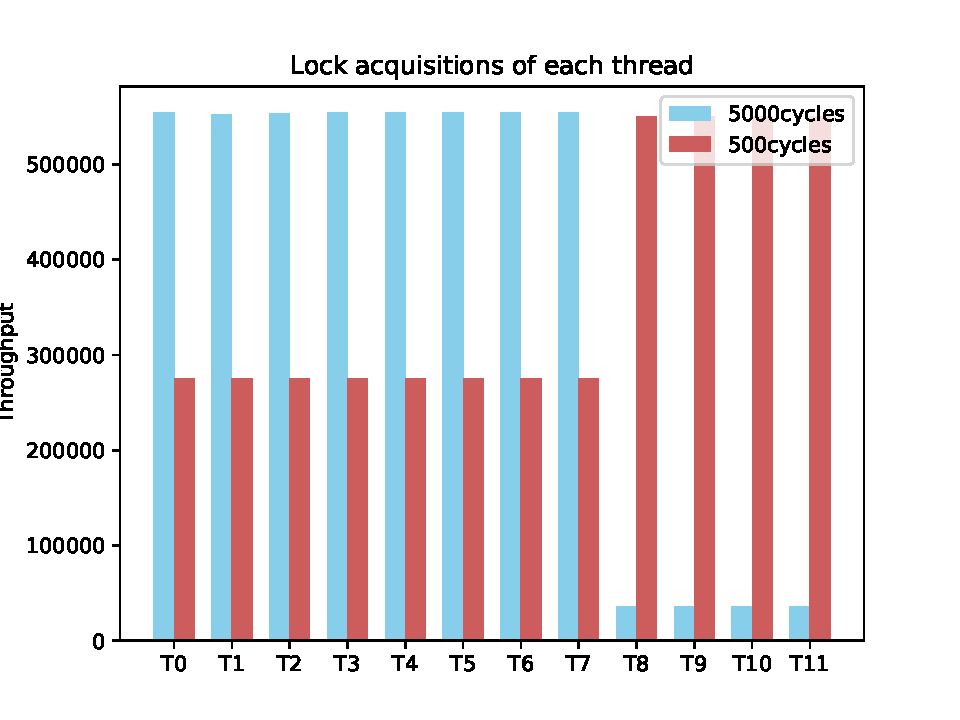
\includegraphics[width=2.8in]{compact.pdf}
\caption{单个线程的吞吐率(紧凑放置)}
	\label{Fig:compact}
\end{minipage}
\begin{minipage}[t]{0.48\textwidth}
\centering
	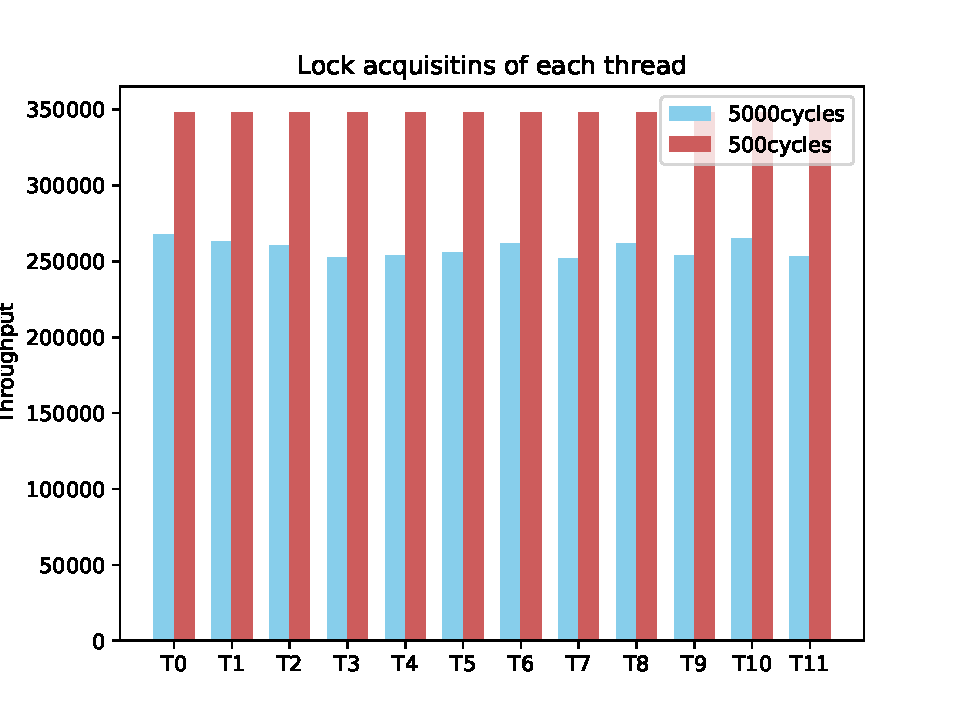
\includegraphics[width=2.8in]{even.pdf}
	\caption{单个线程的吞吐率(平均放置)}
	\label{Fig:even}
\end{minipage}
\end{figure}

综合以上实验现象可以看出,基于队列的层级锁的吞吐率(性能)及其在线程间的分布(长期公平性)与线程放置策略和锁的竞争强度都有关,所以下一小节我们将以实验中的C-MCS锁为例,考虑上述两个因素的基础上结合基于队列的层级锁的锁传递规则对其的性能和长期公平性进行建模来分析影响基于队列的层级锁的性能和长期公平性的根本因素。

\section{模型}
这一小节中,我们先给出几个合理的模型假设,然后将线程在节点上的分布表示为约束并将全局MCS锁在相关节点上各传递一次的间隔作为衡量吞吐率和长期公平性的一个统计周期,在此基础上对吞吐率和长期公平性进行建模。
\subsection{模型假设}
我们在本模型中做三点假设:1)每个线程被放置在一个专用的核上,即每个节点上放置的线程数不应该超过该节点上的计算核心数,从而避免锁的持有者或者等待者被抢占所带来的问题;2)层级锁的竞争较为激烈且至少已经饱和;3)每个线程执行相同的任务:执行非关键区域、请求锁、拿锁、执行关键区域、放锁,并且短期内同一个线程的关键区域和非关键区域的执行时间是不变的。上述第一点假设是现有层级锁中比较通用的做法,第二点是层级锁比较常见的应用场景,第三点假设只是为了简化模型说明,并不影响该模型的通用性。
\subsection{线程分布}
我们用N表示竞争锁的线程数,用CORES\_PER\_NODE表示每个节点上的计算核心数,这N个线程分布在S个节点上,大小为S数组Count中每个元素Count[i]表示节点i上放置的线程数,则总线程数的约束为
\begin{equation}\label{Eq:threads}
  \sum_{i=1}^{S} Count[i] = N
\end{equation}
对于1到S每个节点i上放置的线程数Count[i]有约束
\begin{equation}\label{Eq:non-zero}
  0 < Count[i] <= CORES\_PER\_NODE
\end{equation}
由式\ref{Eq:threads}和式\ref{Eq:non-zero}可得
\begin{equation}\label{Eq:S}
  S >= \lceil\frac{N}{CORES\_PER\_NODE}\rceil
\end{equation}
线程放置策略决定了S的大小及Count数组中每个元素的大小,只需满足上述两个约束即可。

\subsection{统计周期}
C-MCS锁中用到的全局锁和本地锁都是MCS锁,而MCS锁按照先进先出(FIFO,first in first out)的顺序在线程之间传递,所以我们可以认为全局MCS锁在相关NUMA节点之间按照Round-Robin的方式传递;对于某个特定节点上的线程来说,当第一个请求者代表该节点拿到全局锁时,对应的本地MCS锁在该节点上运行的所有相关节点之间也按Round-Robin的方式传递,直到最后一个请求者释放全局锁(当前节点没有后续请求者)或者某个请求者被强制释放全局锁(当前节点上的传递次数达到threshold),如图\ref{Fig:circulation}所示。为了说明的方便,我们将全局MCS锁在所有S个相关节点之间传递一次的时间间隔定义为一个循环(circulation),并且以一个循环为单位来评估吞吐率和长期公平性。

\begin{figure}[t]
	\centering
	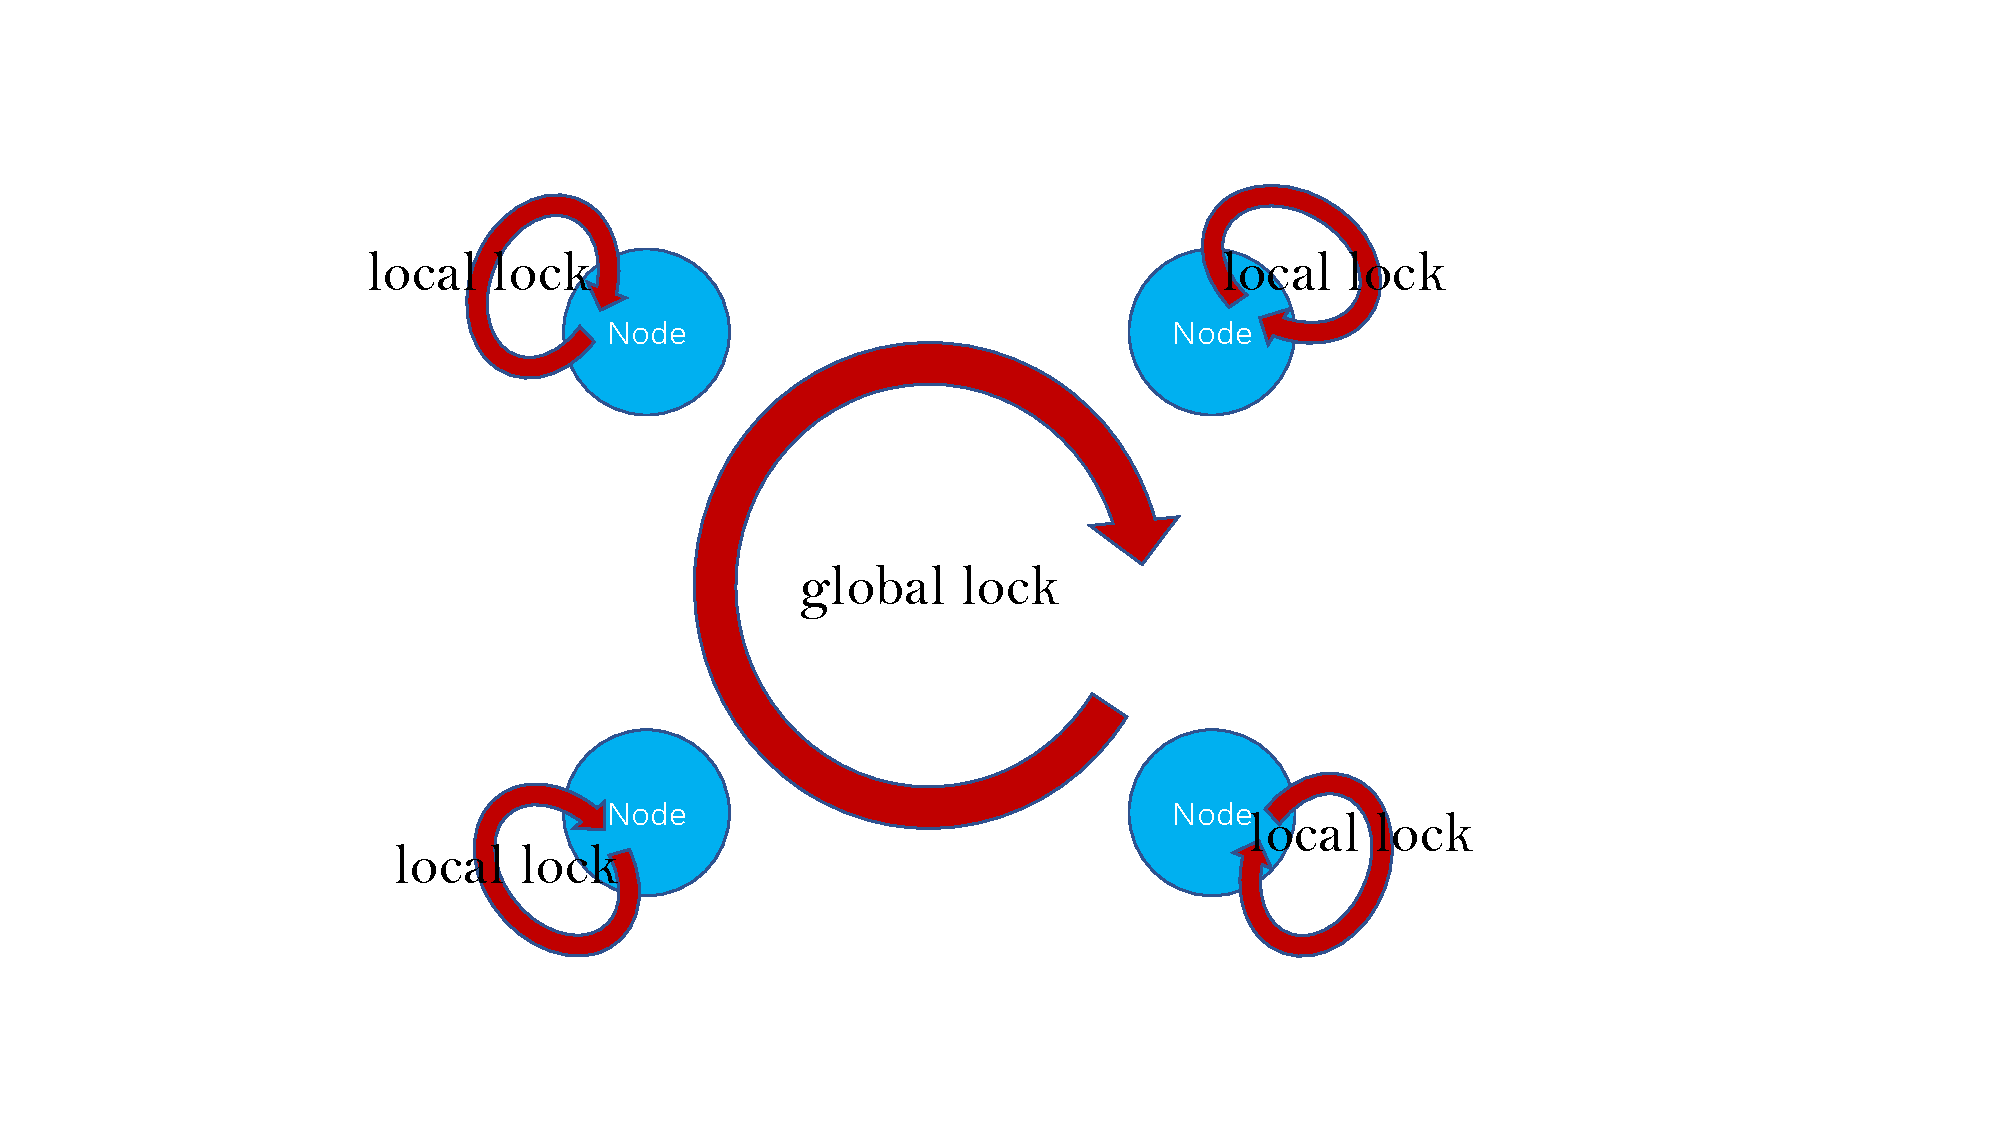
\includegraphics[width=5.6in]{circulation.pdf}
	\caption{C-MCS锁中的一个循环}
	\label{Fig:circulation}
\end{figure}

我们用二维数组Acquisitions来表示单个线程在一个循环内的拿锁次数,其中每个元素Acquisitions[i][j]表示第i个NUMA节点上的线程j在一个循环内的拿锁次数,用interl表示跨节点的锁传递时延,用intral表示同一节点内的锁传递时延(其中一般情况下interl是intral的2-7倍\cite{kashyap2017scalable}),则一个循环的总时间可以表示为
\begin{equation}\label{Eq:duration}
 Duration=\sum_{i=1}^{S}\sum_{j=1}^{Count[i]} Acquisitions[i][j] * intral + S * (interl - intral)
\end{equation}
其中intral和interl之间的数倍的差异在本模型中代表NUMA因素,即访存的非一致性特征。

\subsection{吞吐率}
基于上述定义,一个循环内锁在所有相关节点上所有竞争该锁的线程间总的传递次数可以表示为
\begin{equation}\label{Eq:totalacqui}
  TotalAcquisitions=\sum_{i=1}^{S}\sum_{j=1}^{Count[i]} Acquisitions[i][j]
\end{equation}
进而吞吐率即单位时间内锁在线程间的平均传递次数可以表示为
\begin{equation}\label{Eq:total-thrpt}
 Throughput=\frac{TotalAcquisitions}{Duration}
\end{equation}
由式\ref{Eq:duration}、式\ref{Eq:totalacqui}和式\ref{Eq:total-thrpt}可得
\begin{equation}\label{Eq:thrpt-new}
 Throughput=\frac{1}{1+S*(interl - intral)/TotalAcquisitions}
\end{equation}
其中interl和intral由机器的物理特征决定的,可以认为是常量。所以要获得更高的吞吐率,应该使TotalAcquisitions尽可能地大,S尽可能地小。其中S还要满足式\ref{Eq:S}的约束。

\subsection{长期公平性}
如前所述,我们用一个循环内各个线程拿锁次数的变异系数来衡量基于队列的层级锁的长期公平性,变异系数越小,长期公平性越好。一个循环内每个线程的平均拿锁次数为
\begin{equation}\label{Eq:AVG}
  \mu = \frac{TotalAcquisitions}{N}
\end{equation}
标准差为
\begin{equation}\label{Eq:SD}
  \sigma=\sqrt{\frac{\sum_{i=1}^S\sum_{j=1}^{Count[i]}(Acquisitions[i][j]-\mu)^2}{N}}
\end{equation}
从而变异系数可以表示为
\begin{equation}\label{Eq:CV}
 c_v=\frac{\sigma}{\mu}
\end{equation}
由上述公式及长期公平性的物理意义都可以看出,要获得更好的长期公平性应该使得长远来看每个线程的拿锁次数尽可能地接近,即Acquisitions数组中的元素应该尽可能接近。

\subsection{一个统计周期内单个线程的拿锁次数}
从上述对吞吐率和长期公平性地建模可以看出两者都在很大程度上由Acquisitions数组即单个线程在一个循环内的拿锁次数决定,所以以下我们按照C-MCS锁的传递规则对一个循环内每个线程的拿锁次数进行建模。在此之前我们先定义和说明锁的竞争强度及饱和点,因为Acquisitions数组中的元素的大小和线程放置及锁的饱和点有关,以下将会对此进行详细说明。

\subsubsection{锁的竞争强度及饱和点}
我们定义锁的竞争强度为任何时刻执行关键区域或者等待进入关键区域的线程数的期望,该期望越大,表明锁被请求得越频繁,锁的竞争强度越高。由定义可知锁的竞争强度由两个因素决定:1)竞争者的数量,即竞争同一个锁的线程数,本模型中为N;2)单个竞争者中关键区域执行时间在总执行时间中的占比。单个竞争者的关键区域执行时间在总执行时间中的占比可以表示为
\begin{equation}\label{Eq:pro}
     ratio = CS / (NCS + CS)
\end{equation}
其中CS和NCS分别代表关键区域和非关键区域的长度。基于此锁的竞争强度可以用下式表示
\begin{equation}\label{Eq:expectation}
     competition = N * ratio
\end{equation}
当competition恰好等于1时,锁被持续持有并且所有线程无需等待就能在请求锁的时候就拿到锁,即此时锁恰好饱和\cite{dice2017malthusian},此时的线程数即锁当前饱和点的大小Sat,由式\ref{Eq:pro}和式\ref{Eq:expectation}并且令competition为1可得
\begin{equation}\label{Eq:sat}
     Sat = (NCS + CS) / CS
\end{equation}
在本模型中,Sat的意义主要在于:当一个NUMA节点上放置的线程数达到或者超过Sat时,该节点上的任何一个线程放锁后,该节点上总有至少一个其他线程在等待锁,则按照基于队列的层级锁的锁传递规则,锁将连续在该节点上的线程之间传递直到当前循环内锁在该节点上总的传递次数达到预先设定的threshold为止。

\subsubsection{单个线程的拿锁次数}
在锁的饱和点和基于队列得层级锁的传递规则的基础上,我们现在考虑单个线程在一个循环内的拿锁次数。在每一个循环中,如果NUMA节点i上放置的线程数Count[i]大于等于饱和点Sat,则节点i上的任何一个线程在放锁时总是至少有一个i上的其他线程在等待锁,所以锁会在该节点上一直传递直到节点i上总的传递次数达到预先设定的上限threshold;否则节点i上的最后一个线程放锁后其他线程还在执行非关键区域,此时一个循环内锁在该节点上的传递次数为Count[i]。即
\begin{equation}\label{Eq:localtrans}
local\_acquisitions =
\begin{cases}
Count[i] &\text{Count[i] < Sat}\\
threshold &\text{otherwise}
\end{cases}
\end{equation}
因为每个节点上的本地MCS锁是完全公平的,所以我们可以认为同一个节点上的每个线程的在一个循环内的拿锁次数相等,即节点i上每个线程j在一个循环里边的拿锁次数为
\begin{equation}\label{Eq:per}
Acquisitions[i][j] =
\begin{cases}
1 &\text{Count[i] < Sat}\\
\frac{threshold}{Count[k]} &\text{otherwise}
\end{cases}
\end{equation}
一般情况下为了获取更高的吞吐率,threshold通常被设为Count[k]的若干倍,所以每个节点上放置的线程能否使该节点上的本地锁饱和对于该节点上的每个线程在一个循环内的拿锁次数影响很大。

由式\ref{Eq:localtrans}和式\ref{Eq:per}可以得出以下基本结论
\begin{enumerate}
    \item 由于每个节点上的本地MCS锁是绝对公平的,所以一个循环内同一个节点内的线程的拿锁次数理论上是相等的,即放置在同一个NUMA节点上的线程之间不存在长期不公平的问题;
    \item 一个循环内两个不同NUMA节点上的线程是否长期公平由这两个节点上放置的线程数是否相等决定;
    \item 节点k上放置的线程数Count[k]与饱和点Sat的关系决定了一个循环内节点k上每个线程的拿锁次数是1还是$\frac{threshold}{Count[k]}$,并且这两者之间通常是数倍的关系。
\end{enumerate}
上述结论解释了本章开头的实验中两中线程放置策略对应的吞吐率差异和其在线程间的分布差异。紧凑放置中两个NUMA节点上放置的线程数不相等所以两个NUMA节点上的线程间吞吐率差异巨大,而紧凑放置保证了至少有一个节点上的本地锁饱和所以其对应的吞吐率较高。平均放置中两个NUMA节点上放置的线程数相等所以所有吞吐率在所有线程间的分布较为均匀,在竞争较小时(此时Sat较大)平均放置后两个NUMA节点上的本地锁都未能饱和所以对应的吞吐率较小。

为了后续论述长期公平性的方便,我们定义两个线程之间的关系为对 称(symmetric)如果不管锁的竞争强度如何变化,这两个线程理论上长期的拿锁次数相等。由上述建模及分析可知,运行在同一个NUMA节点上的任何两个线程之间是对 称的;而对于运行在两个不同节点上的线程来说,当这两个节点上运行的线程数量相等时,这两个线程是对称的。显然,对称关系是一种等价关系,因此所有竞争同一个层级锁的线程可以按照其在 NUMA 节点上的分布来被分为若干等价类。

\section{挑战分析}

由式\ref{Eq:thrpt-new}可知为了使基于队列的层级锁获得高吞吐率,S(有线程分布的NUMA节点数)应该尽可能地小而TotalAcquisitions(一个循环内总的锁传递次数)应该尽可能地大。其中由式\ref{Eq:S}知S满足约束S\,>=\,$\lceil N\,/\,CORES\_PER\_NODE\rceil$,所以为了获得更高高吞吐率,S的值应取$\lceil N\,/\,CORES\_PER\_NODE\rceil$。而由式\ref{Eq:totalacqui}和式\ref{Eq:per}知,为了使TotalAcquisitions尽可能地大,应该保证尽可能多的节点上放置的线程数大于等于Sat。

由式\ref{Eq:AVG}到式\ref{Eq:CV}可知,为了保证长期公平性,应当尽可能地缩小线程之间拿锁次数的差异,而从式\ref{Eq:localtrans}和式\ref{Eq:per}可知同一个NUMA节点内各个线程的拿锁次数理论上是相等的,而只有两个节点上放置的线程数相等时这两个节点上的各个线程的拿锁次数理论上才是相等的。所以保证长期公平性应当使得所有相关节点上放置的线程数相等,即 Count[1]=Count[2]=......=Count[S-1]=Count[S]。
    
此外,线程放置还必须满足上述模型中的式\ref{Eq:threads}和式\ref{Eq:non-zero}的约束,即每个线程必须被放置到一个可用的NUMA节点上且该节点上放置的线程数不应该超过该节点的物理核心数,从而避免锁的持有者和等待着被抢占带来的问题。

上述三点对线程的放置有不同的约束和要求,很多场景下上述三个约束和要求不可能同时满足,也就不可能同时保证基于队列的锁的性能和长期公平性,这是基于队列的层级锁中线程放置面临的一大挑战。另外现实应用中锁的竞争强度(线程数和Sat)会随着时段、热点事件等很多不可控事先很难预测的因素的变化而变化,现有固定的线程放置策略显然不可能在锁的竞争变化的情况下同时保证其性能和长期公平性,这是基于队列的层级锁中线程放置策略面临的另一大挑战。

针对上述两项挑战,我们认为一方面需要有额外的机制来改善现有线程放置策略使得在任何竞争强度下都有能同时保证两者的线程放置策略;另一方面,也需要通过竞争感知来根据锁的竞争强度来应用合适的线程放置策略。所以我们在对现有简单单一地线程放置策略(平均放置和紧凑放置)改进的基础上提出了竞争感知的混合线程放置框架CAH,下一章我们将对CAH的设计与实现做详细介绍。


\section{本章小结}
在这一章中,我们首先说明了锁的性能和长期公平性的衡量标准,接着通过实验展示了基于队列的层级锁中现有的线程放置策略在吞吐率和长期公平性方面的存在的缺陷,然后通过对吞吐率和长期公平性建模分析出了决定基于队列的层级锁的吞吐率和长期公平性的关键因素,最后在此基础山得出了基于队列的层级锁中线程放置策略所面临的挑战:某些场景下不可能同时兼顾性能和长期公平性、不能适应锁的竞争强度动态变化的场景。针对上述挑战,我们对现有线程放置策略进行了改进,并在此基础上提出了竞争感知的混合线程放置框架CAH,下一章将会对CAH的设计与实现做详细说明。